\documentclass[conference]{IEEEtran}
\IEEEoverridecommandlockouts
% The preceding line is only needed to identify funding in the first footnote. If that is unneeded, please comment it out.
\usepackage{cite}
\usepackage{amsmath,amssymb,amsfonts}
\usepackage{algorithmic}
\usepackage{graphicx}
\usepackage{textcomp}
\usepackage{xcolor}
\usepackage{listings}
\lstset{captionpos=b,basicstyle=\footnotesize}

\graphicspath{{../figures/}}
\def\BibTeX{{\rm B\kern-.05em{\sc i\kern-.025em b}\kern-.08em
    T\kern-.1667em\lower.7ex\hbox{E}\kern-.125emX}}
\begin{document}


\title{Disabling Prefetcher to Amplify Cache Side Channels}

%\author{
%    \IEEEauthorblockN{1\textsuperscript{st} Meet Udeshi}
%    \IEEEauthorblockA{\textit{Electrical Engineering Department} \\
%    \textit{Indian Institute of Technology, Bombay}} &
%    \IEEEauthorblockN{2\textsuperscript{nd} Nirmal Kumar Boran}
%    \IEEEauthorblockA{\textit{Electrical Engineering Department} \\
%    \textit{Indian Institute of Technology, Bombay}} &
%    \IEEEauthorblockN{3\textsuperscript{rd} Virendra Singh}
%    \IEEEauthorblockA{\textit{Electrical Engineering Department} \\
%    \textit{Indian Institute of Technology, Bombay}}
%}

\maketitle

\begin{abstract}
Cache side channels are well known for being effective
in extracting data from modern cryptographic ciphers.
Attackers try to generate collisions with a victim program sharing
the same cache, and study their own cache timings to infer the
victim's memory accesses.
%Side channel attacks gather data on their own cache hits and cache misses,
%and can infer a program's memory accesses based on this data.
Some other hardware accessing the cache, e.g. prefetcher, degrades the
quality of the side channel by introducing false positives in the attacker's
data.
This paper describes a method to disable the prefetcher by preventing
it from generating memory accesses and interfering with side channels
running in the cache.
An attacker implementation is designed to work on a Stride Prefetcher.
%This implementation is tested with OpenSSL AES program.
Results show that it is able to significantly reduce the number of prefetches
generated to almost 0.

%Such attacks assume that the victim program is the only other one making accesses
%to the shared cache. Any accesses not originating from the victim program
%lead to false positives which introduces noise in the side channel.
%Attackers can restrict other programs from running on the core and
%synchronize the attack with execution of relevant section of code of the
%victim program. However, they cannot directly switch off hardware units
%like Prefetchers which may generate accesses to the cache.
%This work describes a method in which the prefetcher is prevented
%from generating any accesses using an attack tailored to disable its
%function.
\end{abstract}

\begin{IEEEkeywords}
security, side channels, prefetcher
\end{IEEEkeywords}

\section{Introduction}

 % Side channels look at cache accesses of victim to deduce data
An attacker program using the cache as a side channel tries to force
collisions with the victim program by making accesses which alias to the
same cache lines \cite{osvik-cache-attacks}.
Time taken for subsequent accesses to these cache lines differs and is used to
determine whether there was a successful collision or not.
This data is further used to infer whether the victim accessed a particular
cache line or not, thus leaking data about the data of the program.
 % Prime+Probe determines if victim evicted certain cache set
 % when it's own data is evicted from that cache set. It looks for
 % cache miss.
Different implementations of the side channel look for either a cache
hit or a cache miss as a sign of successful collision.
The Prime+Probe attack fills the cache lines in a set with data other than
that being accessed by the victim. Any access by the victim to that set will
cause attacke's data to be evicted, which will show up during the Probe step
as a cache miss \cite{osvik-cache-attacks}.
 % Flush+Reload tries to get a cache hit on the data victim may have
 % accessed, like a common library.
Similarly, the Flush+Reload attack looks for a cache hit to the same
data as the victim. A cache hit in the Reload step is infered as successful
collision \cite{percival-rsa}.

 % Side channel attacks require least interference, else they will get
 % false positives because an attacker cannot determine where the cache
 % access came from.
 % They can only deduce properly if correct code segment of
 % program is executing, nobody else.
 % Any other entity accessing the cache will interfere
The attacker assumes a scenario where only the victim is making memory
accesses, hence is able to deduce the memory access pattern. If there is
another program or hardware making memory accesses, they will surely
interfere with the side channel. After obtaining a successful collision,
there is no way for the attacker to distinguish whether the source of
this collision was truly the victim. Fuchs et al \cite{fuchs-disruptive}
introduce a Disruptive Prefetcher which generates spurious memory accesses,
making the victim's accesses indistinguishable for any attacker.

 % To reduce interference of prefetcher we try to disable the prefetcher
This paper focuses on a way to disable the prefetcher and significantly reduce
the number of generated prefetches. With a separate attacker focusing on disabling
the prefetcher, it becomes extremely unlikely for the side channel attacker to
see a collision with a prefetcher generated access. This enhances the side channel
and can enable faster and better data retrieval.
 % Work focuses on stride prefetcher but it can be extended to
 % any PC-indexed prefetcher or buffer based prefetcher.
The attack implementation has been designed specific to a Stride prefetcher
\cite{fu-stride}. However, the implementation can be used as-is or easily extended
to apply to any PC-indexed prefetcher table.

% TODO add more to Introduction

\section{Attack Vectors}

 % Stride prefetcher trains on stride value for a certain PC by storing
 % a confidence counter. Disabling prefetcher involves not letting
 % it train on PC values.
 % Some more detail on working of stride prefetcher
 % Prefetcher will be disabled when it does not get to the condition
 % of generating prefetches.
 % They generate prefetch when confidence value crosses threshold.
A Stride Prefetcher tries to identify load instructions which have
a pattern with constant distance between accesses i.e. a fixed stride.
The prefetcher table stores entries containing PC address of the load
instruction, the last accessed memory address, the stride
value and a confidence counter. The table is indexed using the load PC,
which leads to aliasing between multiple PCs.
Higher the value of the confidence counter, higher is the probability that
the next access follows the same stride pattern currently stored.
The prefetcher generates memory accesses when it sees an entry with high
enough confidence. Every entry needs to be prevented from reaching this condition
to disable the prefetcher. This design exposes two attack vectors which the
attacker can use to prevent entries from gaining high confidence.

 % Confidence value is reset below threshold when a new entry is made to the table.
 % This is exploited by periodically making new entries into the table
 % to evict older entries and prevent them from gaining confidence.
 % This attack vector allows us to never let victim's load instruction
 % trigger the prefetcher to generate prefetches.
\textbf{Evict Table Entries:} The attacker can keep creating many new entries
in the table, and the prefetcher will be forced to evict older entries
of the victim which have gained high confidence. When the victim's entry is added
again to the table, it will start from a lower default confidence and will have
to go through the training phase again. If the victim's entry is quickly
evicted by the attacker's entry, it can never gain enough confidence to
generate memory accesses.

 % Confidence is decremented when an entry hits in the table and the stride
 % value does not match. Attacker randomises the stride value in every access.
 % This prevents attacker from generating any prefetches
 % which would be detrimental to the purpose.
\textbf{Decrement Confidence:} The prefetcher calculates the new stride value for
every access using the last address. When this new stride differs from the last stride
stored in the entry, the confidence counter is decremented and the old stride is replaced
with the newly calculated one. This helps to keep confidence low for the attacker's
entries and ensures that there are not accesses generated due to the attacker.

These two attack vectors are utilised to implement an attacker whose target is to
reduce the memory accesses generated by the prefetcher to zero.

\section{Attacker Implementation}

 % To add new entries to Prefetcher table, we need to have a load
 % instruction at new location.
 % A binary is created which contains large number of
 % load instructions placed at different PC addresses so
 % that after aliasing every entry of the prefetcher table is
 % accessed atleast once.
To create new entries in the table, every load executed by the
attacker has to come at a new PC address. A single load inside
a loop will only create one new entry. The attacker binary
is created such that a large number of load instructions
are placed at different PC addresses. There need to be
enough load instructions properly located at different PC addresses
so that, after aliasing, every location in the prefetcher table is accessed
atleast once.

 % Prefetcher is only accessed when there is a cache miss, clflush instruction is
 % used to always generate a cache miss.
It is generally the case that the prefetcher is accessed only
on cache miss. To ensure that the attacker's loads generate a cache miss
the memory address is flushed from the cache hierarchy using \texttt{clflush}
instruction \cite{intel-x86}.


\subsection{Full Attacker}

 % To make load instructions alias to every entry, their PC addresses
 % need to be carefully controlled. The set indexing bits need
 % to attain every possible value enough times to fill all ways.
The full attacker is designed in a way to target the whole prefetcher table,
without considering the victim program running. It targets to disable every
entry in the table by keeping the confidence value low.
Multiple load instructions have to be placed at different PC addresses
so that each entry in the table is aliased to atleast once.
Considering a set-associative table, the set-indexing bits of the PC
are identified.
 % Single load is 4 bytes in X86. accompanying clflush is 3 bytes.
 % sequence of 7 bytes placed one after other will skip certain
 % set indexes. A particular set index may have many loads aliasing
 % to it while another may have very few.
 % To properly control, padding with nop instruction is required.
 % Describe why 8 byte sequence and sequence length + nop
Single load instruction in x86 is of 3 bytes. The corresponding \texttt{clflush}
instruction is of 4 bytes. An extra \texttt{nop} instruction has been added
with the pair to round up the PC increment to 8 bytes.
A large enough sequence of these set of instructions, with extra \texttt{nop}
instructions wherever required, is generated to ensure aliasing
to every entry in the table. It is important that each entry gets a nearly
equal number of hits from the attacker, to be properly effective. The size of
8 bytes of the set of instructions helps in this versus 7 bytes.

\begin{lstlisting}[caption={Full Attacker disassembly: load misses at different PCs},
label={lst:full_attack}]
00000000000006ca <attack>:
  ...
 6ce: 8b 58 36     mov    0x36(%rax),%ebx
 6d1: 90           nop
 6d2: 0f ae 78 36  clflush 0x36(%rax)
 6d6: 8b 58 08     mov    0x8(%rax),%ebx
 6d9: 90           nop
 6da: 0f ae 78 08  clflush 0x8(%rax)
 6de: 8b 58 3f     mov    0x3f(%rax),%ebx
 6e1: 90           nop
 6e2: 0f ae 78 3f  clflush 0x3f(%rax)
 6e6: 8b 58 38     mov    0x38(%rax),%ebx
 6e9: 90           nop
 6ea: 0f ae 78 38  clflush 0x38(%rax)
 6ee: 8b 58 20     mov    0x20(%rax),%ebx
 6f1: 90           nop
  ...
\end{lstlisting}

 % This is called the full attacker because it targets the
 % entire prefetcher table.
Listing \ref{lst:full_attack} shows a part of the disassembly of the binary
generated.
The full attacker takes time to run a single iteration of the attack
because of the repeated cache misses.
An attacker targeting a 16-set 4-way prefetcher table requires
128 load instructions. When each of these loads gives a cache miss,
the latency of the attacker becomes very high.
 % It is possible (and also observed) that some load addresses of the victim
 % can retrain the prefetcher while one iteration is running and generate
 % prefetches.
While one iteration of the attack is running, it is possible that
some of the victim's loads can re-enter the table and build up a high enough
confidence to generate prefetches. This will be seen in the results in Section
\ref{sec:results}.
 % These retrained load instructions will only be evicted in the next iteration.

\subsection{Targeted Attacker} \label{sec:identify-loads}

A faster implementation is required which can quickly evict such notorious loads
of the victim program.
 % If such loads are identified in advance, an attacker which targets the
 % sets of only such loads will be required.
 % Loads can be identified by looking at memory access patterns of the victim
 % program by running simulations with multple random inputs.
When the victim program is known, it is possible to predict which loads will
be able to re-train the prefetcher very quickly. The victim program
is simulated and its memory access pattern is recorded. This pattern when
applied to a simulated model of the prefetcher gives an idea about the
load instructions which are likely generate the most prefetches.
The targeted attacker is tailored to these load instructions and leaves
the rest of the prefetcher entries untouched.
 % From the full attacker we can leave relevant load instructions which
 % alias with the targeted PCs, filter out others by replacing them with nop.
The targeted attacker is generated by filtering out unnecessary load instructions
from the full attacker binary and replacing them by \texttt{nop} instructions.
This leads to a binary with few load instructions scattered and filled with \texttt{nop}
slides.
 % for targeting 2 PCs the number of load instructions required reduces from 256 to 16
A binary generated for hitting 2 load instructions of the victim requires
16 loads compared to the 128 loads of the full attacker. This reduces the
latency of the attacker significantly and makes the attacker
more effective against a victim program with few notorious loads.

\begin{lstlisting}[caption={Targeted attacker disassembly: loads at aliased PCs},
label={lst:targeted_attack}]
00000000000006ca <attack>:
     ...
 6d9: 90           nop
 6da: 8b 58 0f     mov    0xf(%rax),%ebx
 6dd: 0f ae 78 0f  clflush 0xf(%rax)
 6e1: 90           nop
 6e2: 90           nop
 6e3: 90           nop
 6e4: 8b 58 3c     mov    0x3c(%rax),%ebx
 6e7: 0f ae 78 3c  clflush 0x3c(%rax)
 6eb: 90           nop
 6ec: 90           nop
     <nop slide> ...
 6f7: 90           nop
 6f8: 8b 58 2f     mov    0x2f(%rax),%ebx
 6fb: 0f ae 78 2f  clflush 0x2f(%rax)
 6ff: 90           nop
     ...
\end{lstlisting}

Listing \ref{lst:targeted_attack} shows a part of the disassembly of the targeted
attacker binary.
 % The nop slides although important do not add any significant delay
 % compared to the cache misses of load instructions.
The \texttt{nop} slides look like they would add some delay in between but
that is masked by the cache miss latency caused by the load instruction.

\section{Simulation}

\begin{figure}
    \centering
    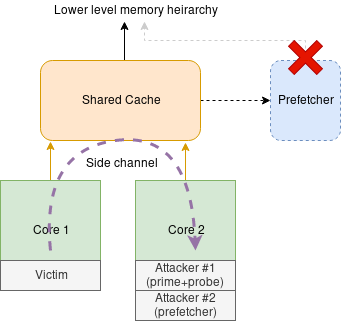
\includegraphics[width=\columnwidth]{prefetch_attack}
    \caption{Setup of attack to disable prefetcher from generating memory accesses}
    \label{fig:prefetch_setup}
\end{figure}

Table \ref{tab:simulation_setup} shows the configuration of
the simulator and included hardware.
% \item Gem5 X86 simulator.
% \item 2x O3 CPUs.
% \item 32kB L1 caches private to each core.
% \item 256kB L2 cache shared between cores.
% \item 64 entry Stride prefetcher for L2, with 16-set 4-way table.
%\end{itemize}
 % Victim program runs on core 1 and attacker runs on core 2
The victim program runs on core 1 and attacker runs on core 2.
The simulator makes measurements for a phase of certain number of instructions.
It records the number of prefetches issued, average confidence of the entries,
hits and misses to the prefetcher table by victim program.
 % Simulator measures number of prefetches issued, average confidence,
 % hits and misses to table
 % These are measured for every 1 million instructions

\begin{table}[hbp]
\centering
\begin{tabular}{|l|r|}
    \hline
    Simulator  & gem5 X86\\
    \hline
    Core Type  & O3 CPUs 8-wide fetch\\
    \hline
    Number of Cores & 2\\
    \hline
    L1 Icache & 32K 8-way\\
    \hline
    L1 Dcache & 32K 8-way\\
    \hline
    L2 cache & 256K 16-way shared between cores\\
    \hline
    L2 prefetcher  & Stride 64-entry 4-way, confidence threshold 4\\
    \hline
\end{tabular}
\\
\caption{Simulation setup}
\label{tab:simulation_setup}
\end{table}

\section{Results} \label{sec:results}

\begin{figure}[htbp]
    \centering
    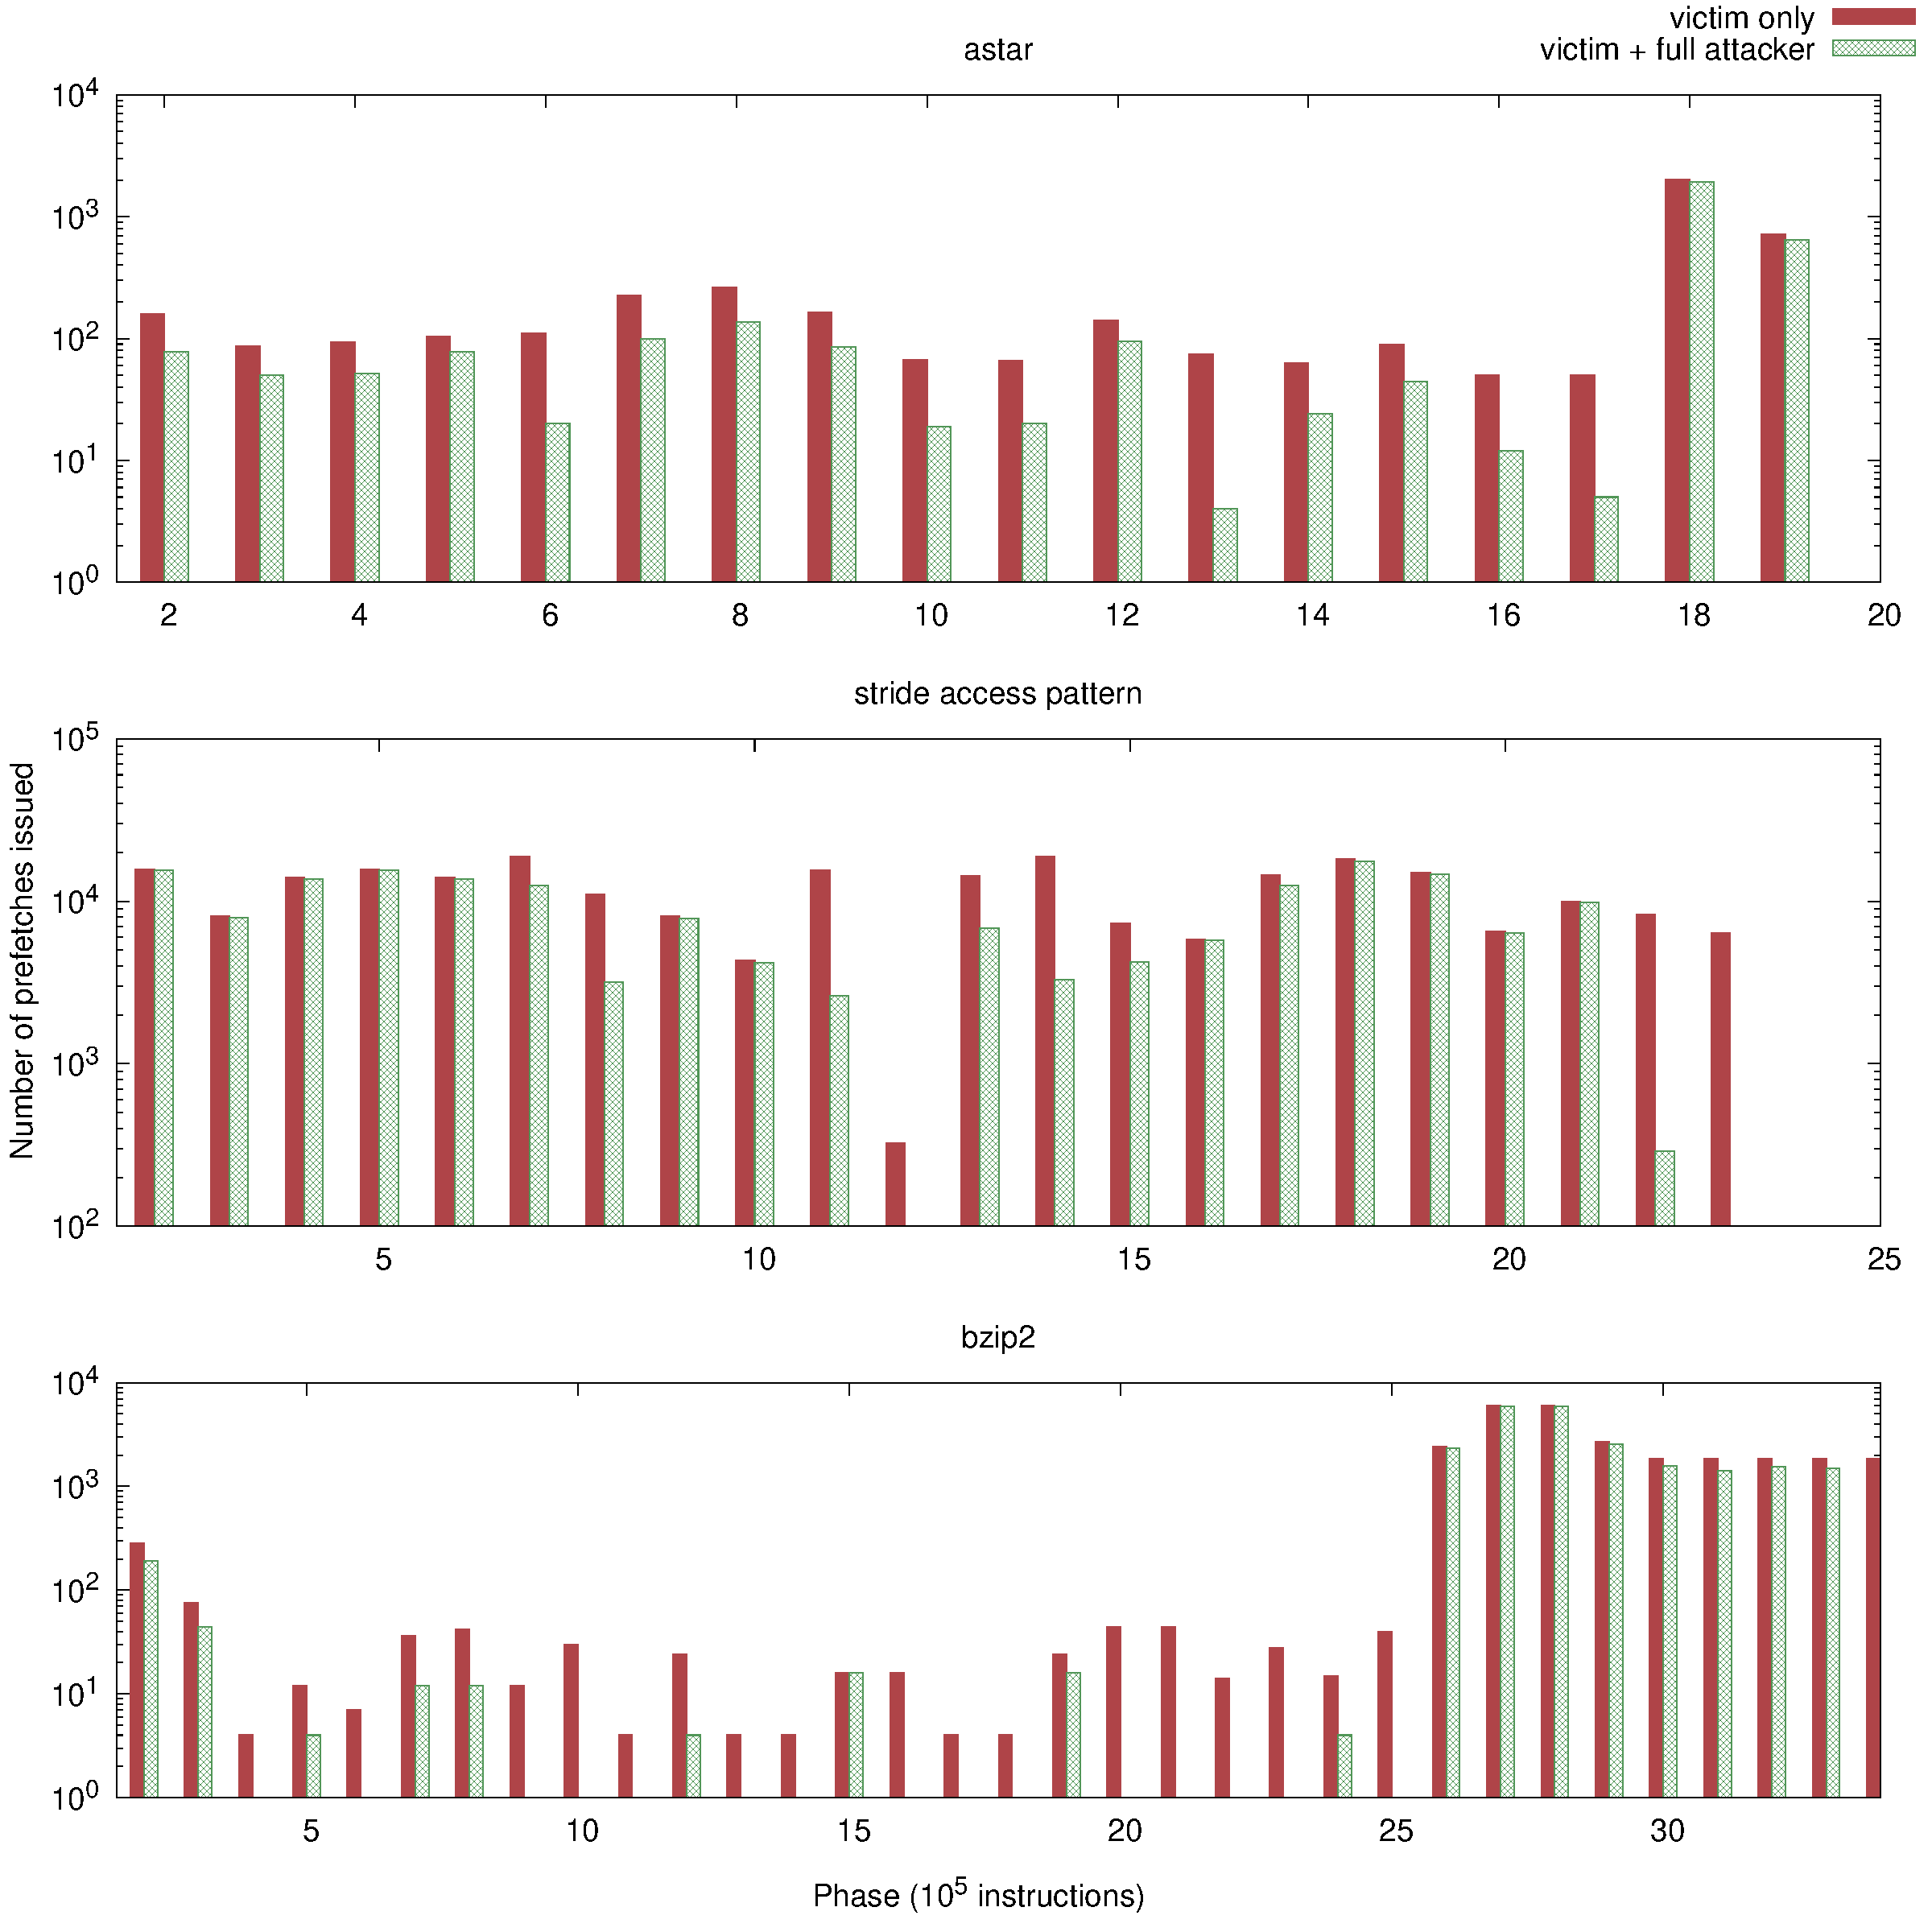
\includegraphics[width=\columnwidth]{hwpf_num}
    \caption{Number of prefetches issued on different benchmarks}
    \label{fig:prefetch_attack}
\end{figure}

\begin{figure}[htbp]
    \centering
    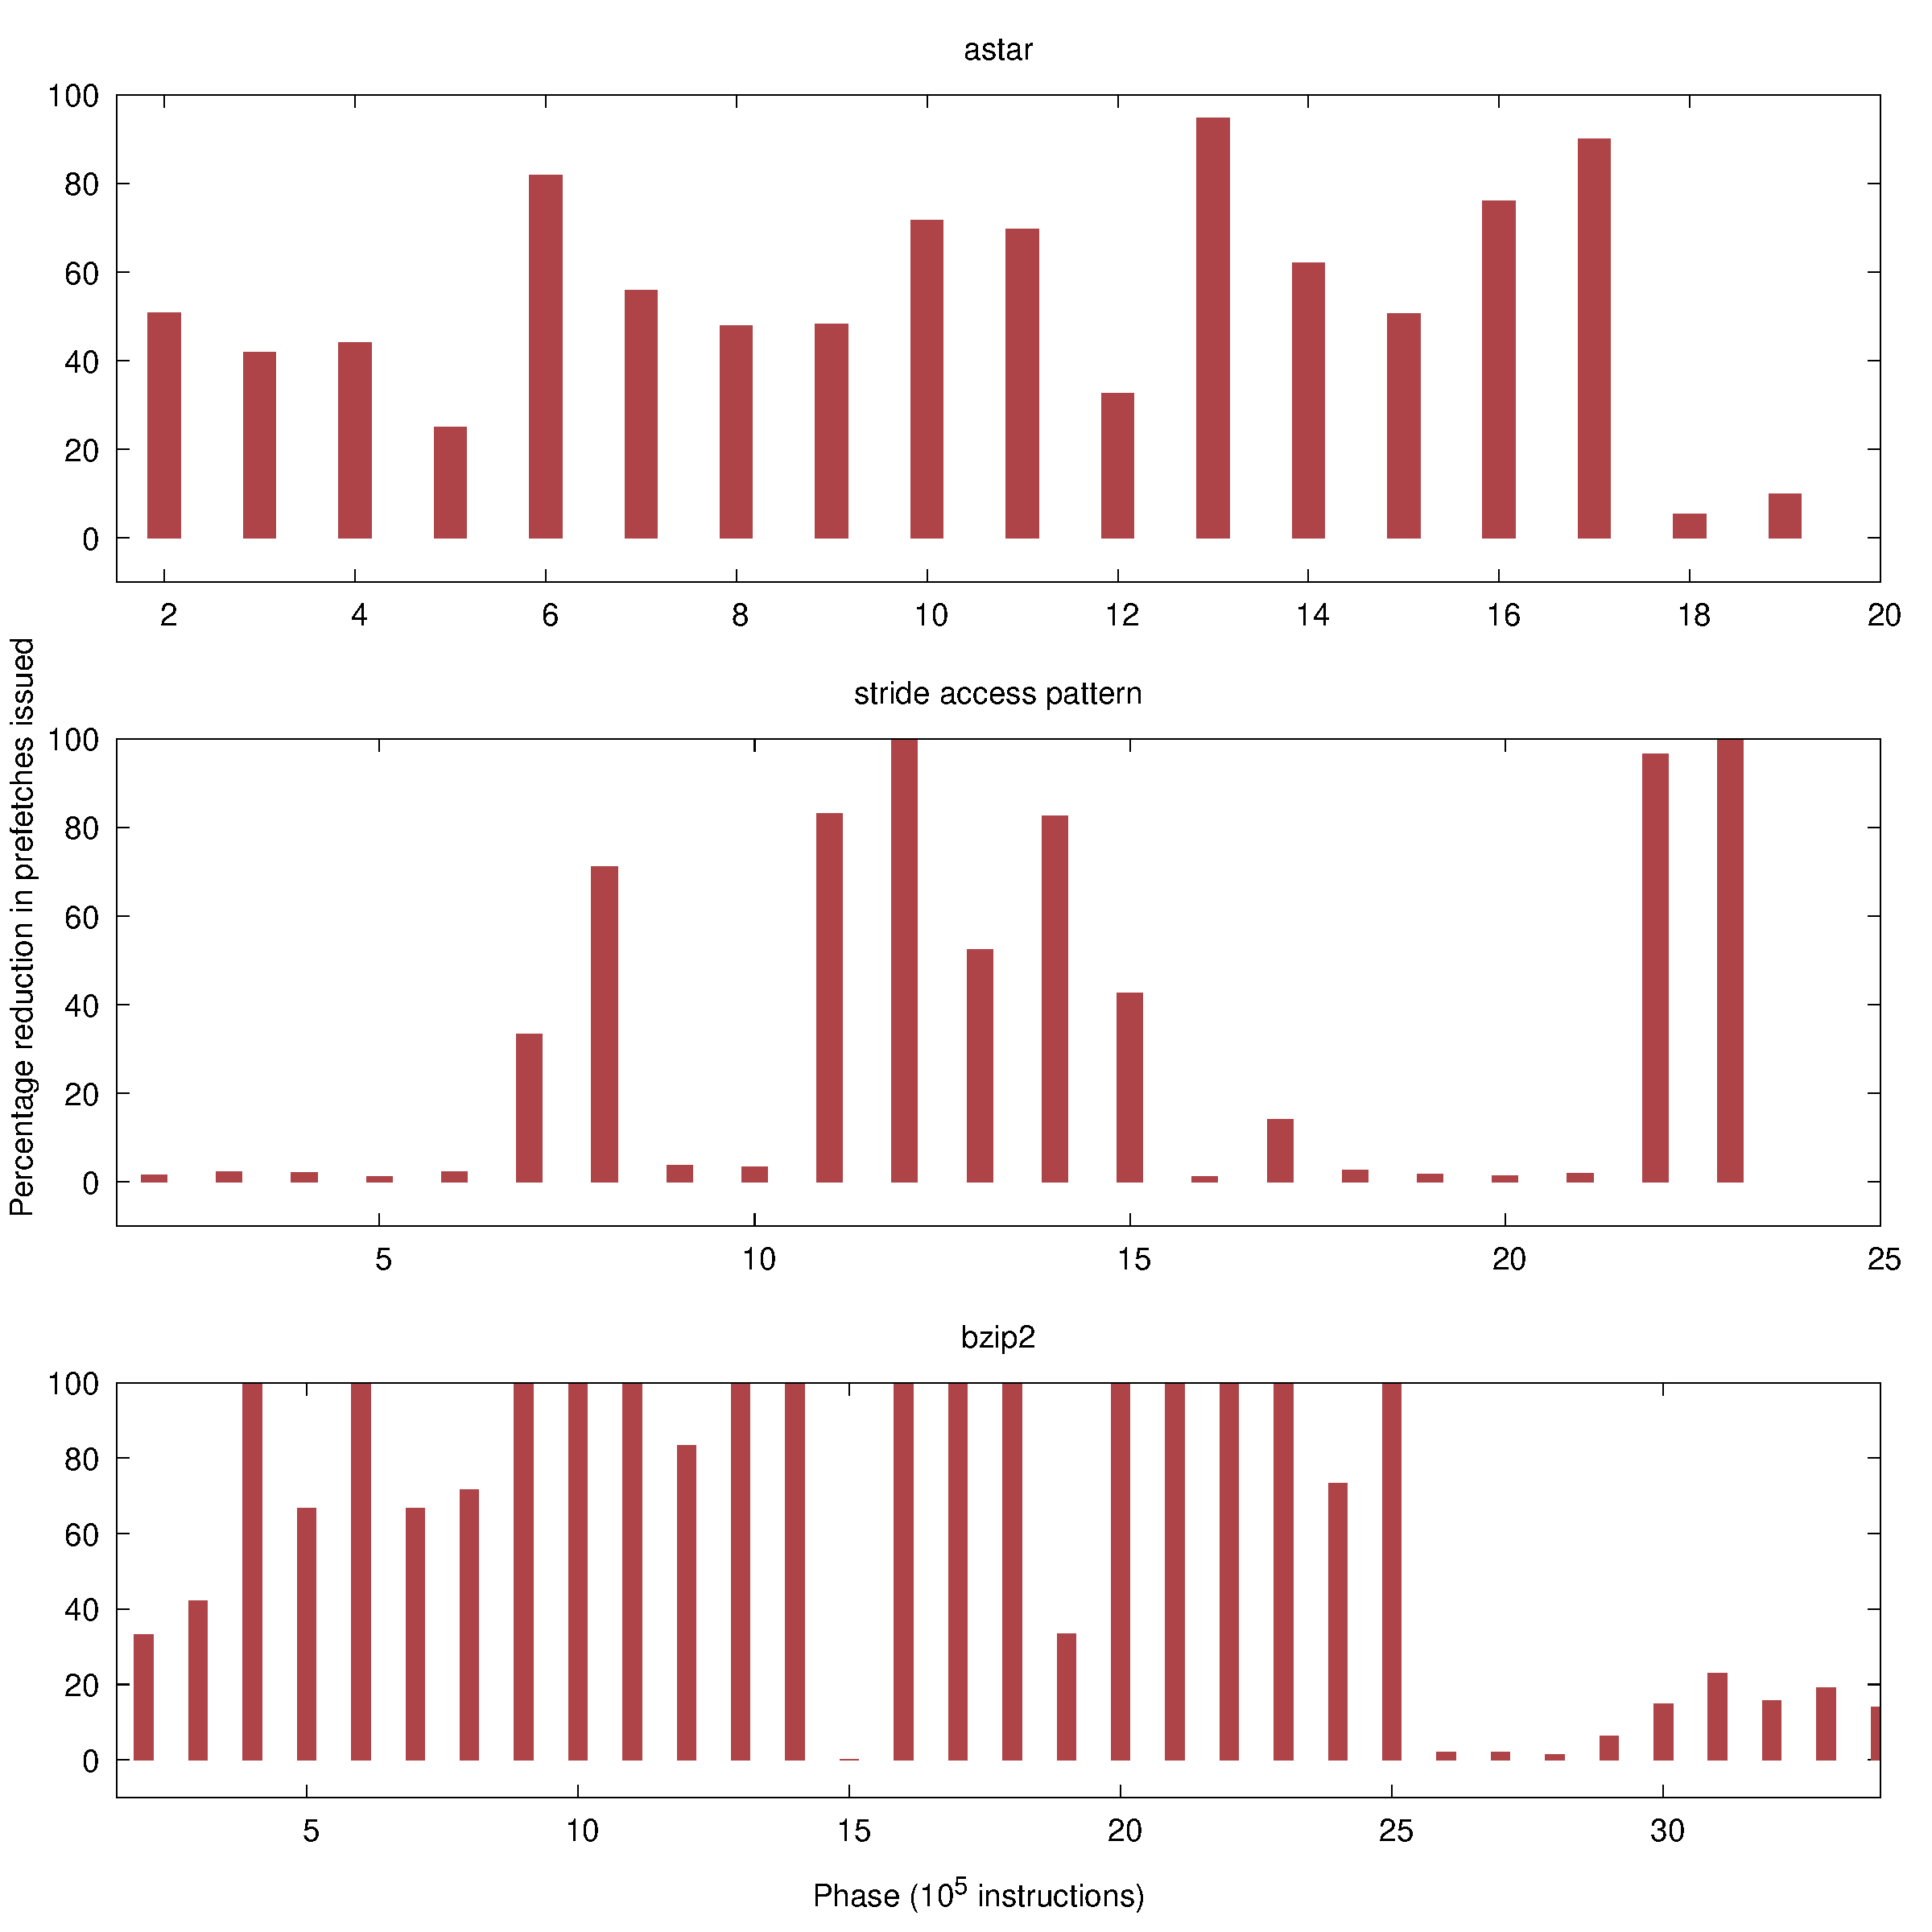
\includegraphics[width=\columnwidth]{hwpf_perc}
    \caption{Percentage reduction in number of prefetches}
    \label{fig:prefetch_percred}
\end{figure}

 % Benchmarks show full attacker is effective against some types of memory access
 % patterns while others are not reduced much.
Figures \ref{fig:prefetch_attack} and \ref{fig:prefetch_percred} show
results of testing the full attacker with a benchmark programs \textit{astar},
\textit{bzip2} and a sample program \textit{stride access generator}.
It is evident that the full attacker is not very effective in some
conditions of the program, which is unacceptable.

\begin{figure}[htbp]
    \centering
    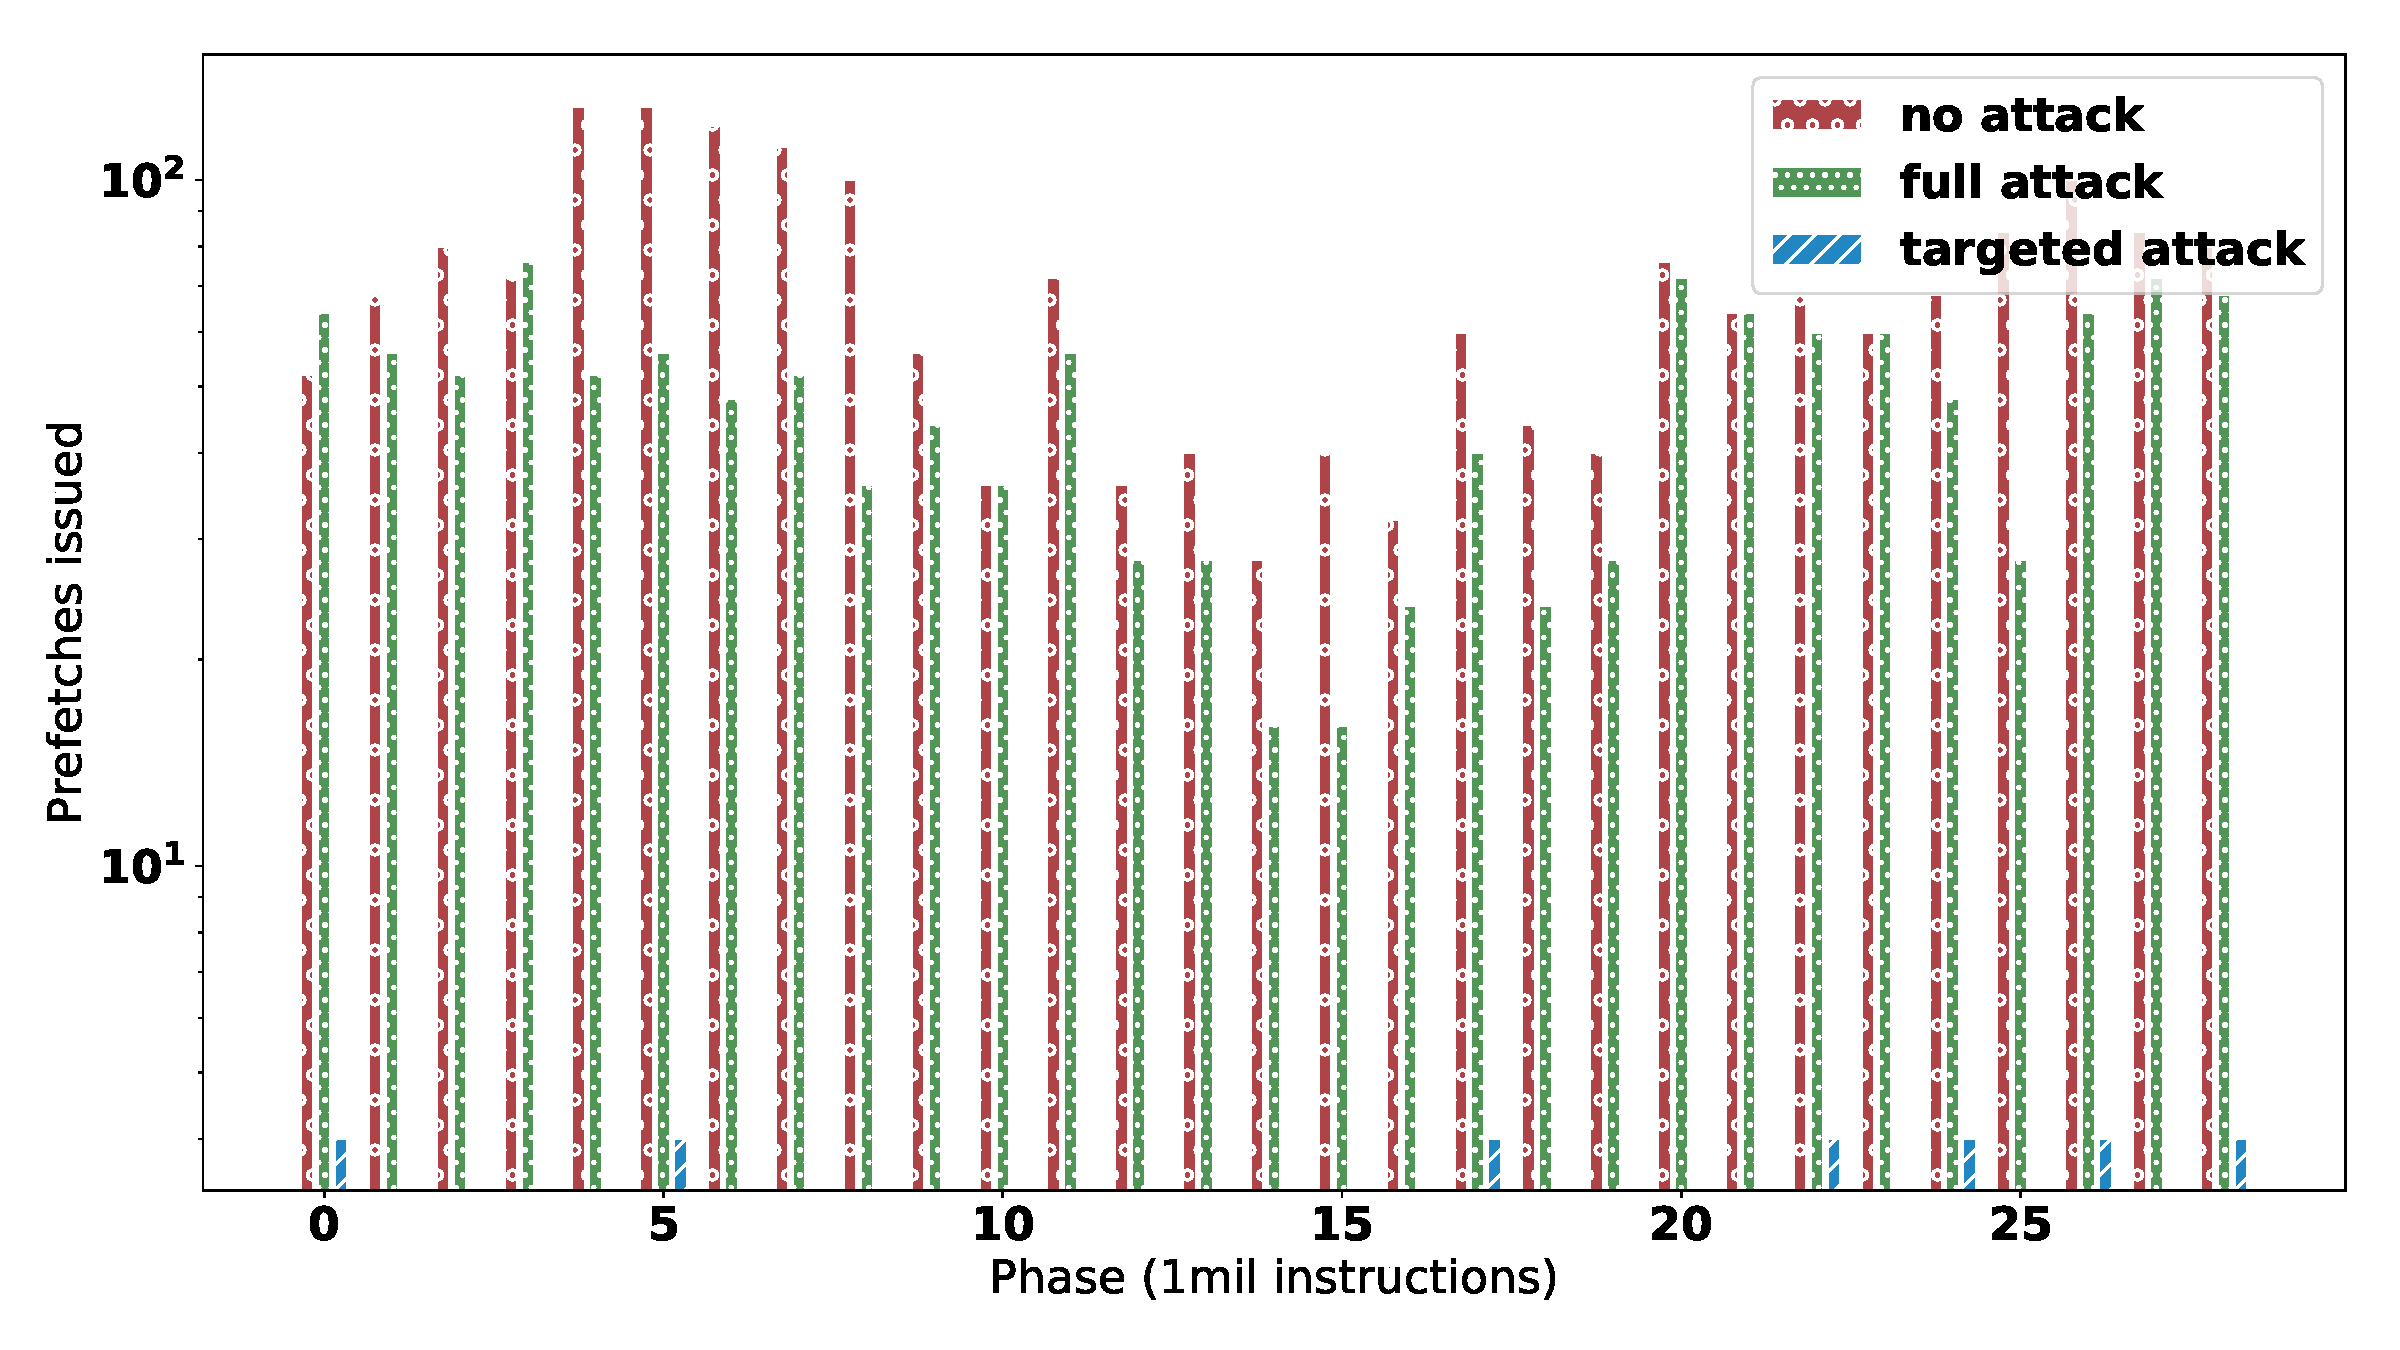
\includegraphics[width=\columnwidth]{pf_issued}
    \caption{Comparision of number of prefetches issued by AES program}
    \label{fig:targeted_attack}
\end{figure}

 % AES victim is implemented which encrypts random data using AES implementation
 % of openssl 0.9.x (uses libcrypto)
For more relevant results, further tests are conducted with the OpenSSL
implementation of AES algorithm. The AES library function is run repeatedly
with random inputs and the same key. The results under various attack
scenarios are measured and compared in Figures \ref{fig:targeted_attack},
\ref{fig:targeted_avgconf} and \ref{fig:targeted_hitrate}.
 % Simulation of only victim helps identify two load addresses which generate
 % most of the prefetches.
Two load instructions are identified for AES victim by using the method outlined
in Section \ref{sec:identify-loads}. The targeted attacker is tailored to those load PCs.
 % Full attacker is somewhat effective at reducing prefetches is some phases,
 % but targeted attacker is extremely effective.
The main observation in Figure \ref{fig:targeted_attack} is that the targeted attacker
is significantly more effective than the full attacker. The full attacker is
able to achieve an average reduction of 32\%, while the targeted attacker is able
to successfully reduce the prefetches to 0.
 % The targeted attacker and full attacker are able to equally reduce confidence
 % of prefetcher
In Figure \ref{fig:targeted_avgconf}, the average confidence of the 2 sets which targeted
prefetcher is attacking is shown. The average confidence with no attacker is 6.9,
with full attacker is 5.2 and with targeted attacker is 3.5. The targeted attacker
is able to lower confidence below the threshold value of 4 hence is successful
in reducing the prefetches.

\begin{figure}[htbp]
    \centering
    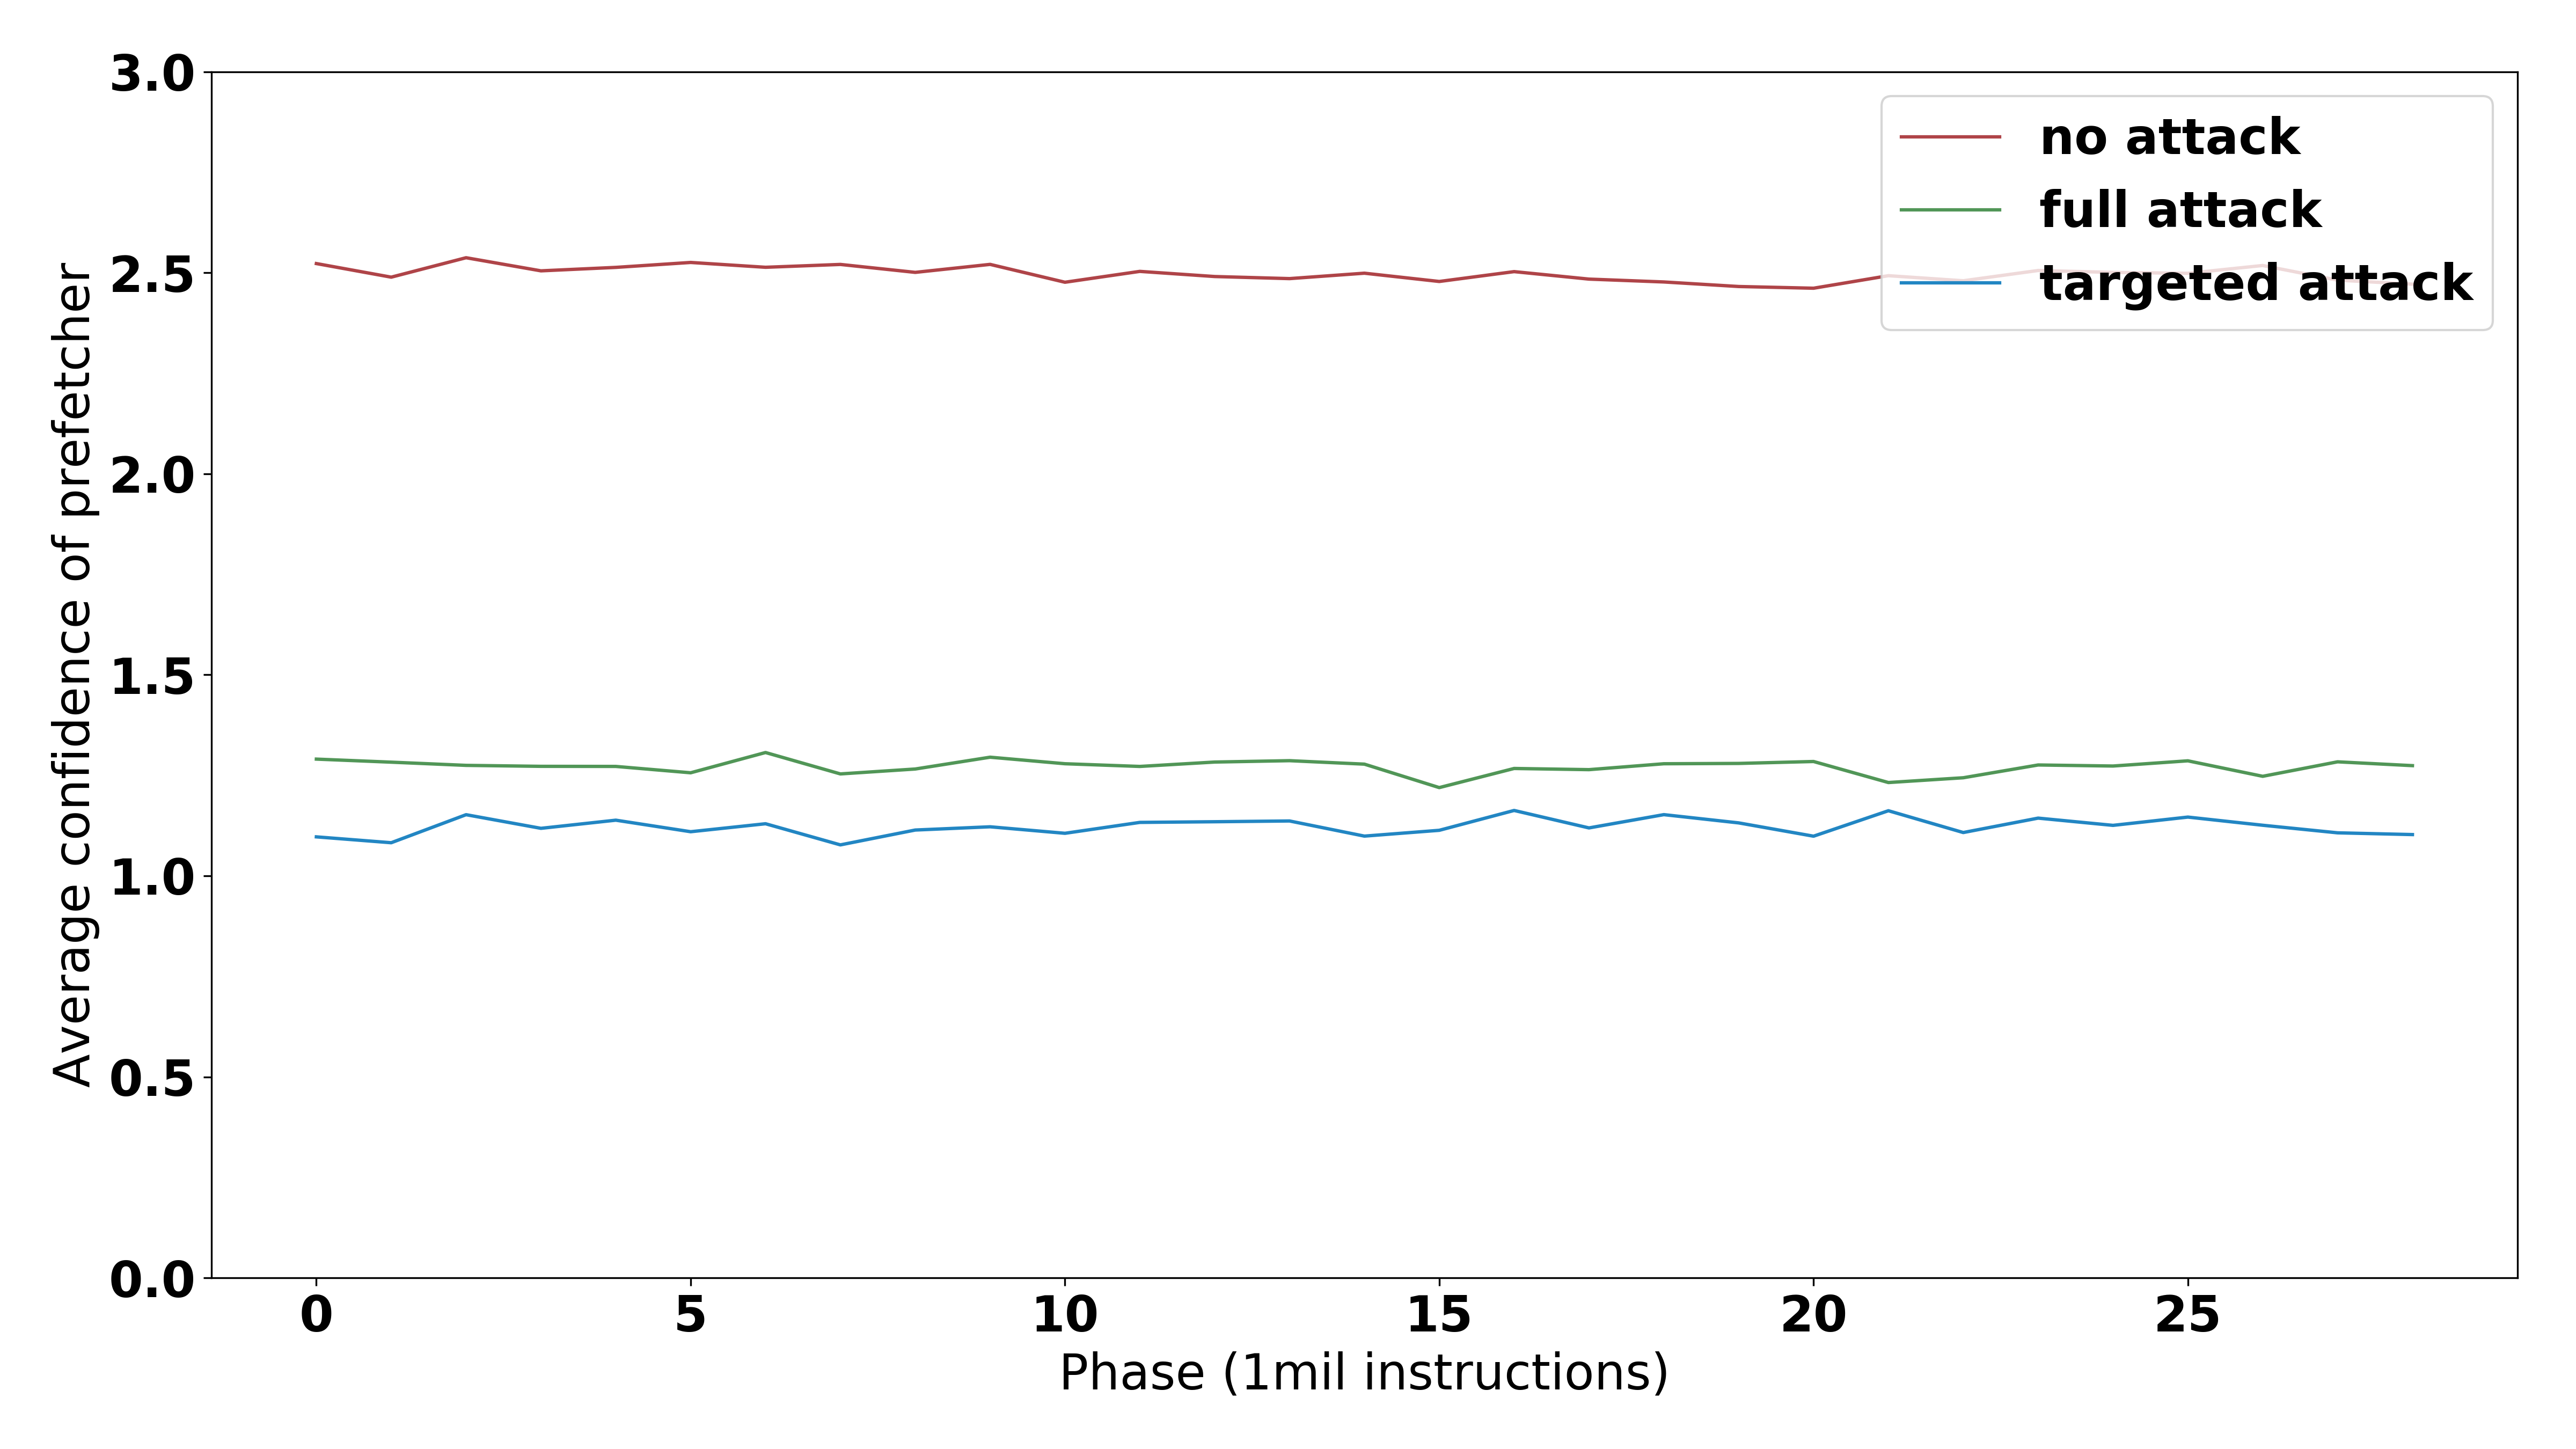
\includegraphics[width=\columnwidth]{avg_conf}
    \caption{Comparision of average confidence of prefetcher with AES program}
    \label{fig:targeted_avgconf}
\end{figure}

\begin{figure}[htbp]
    \centering
    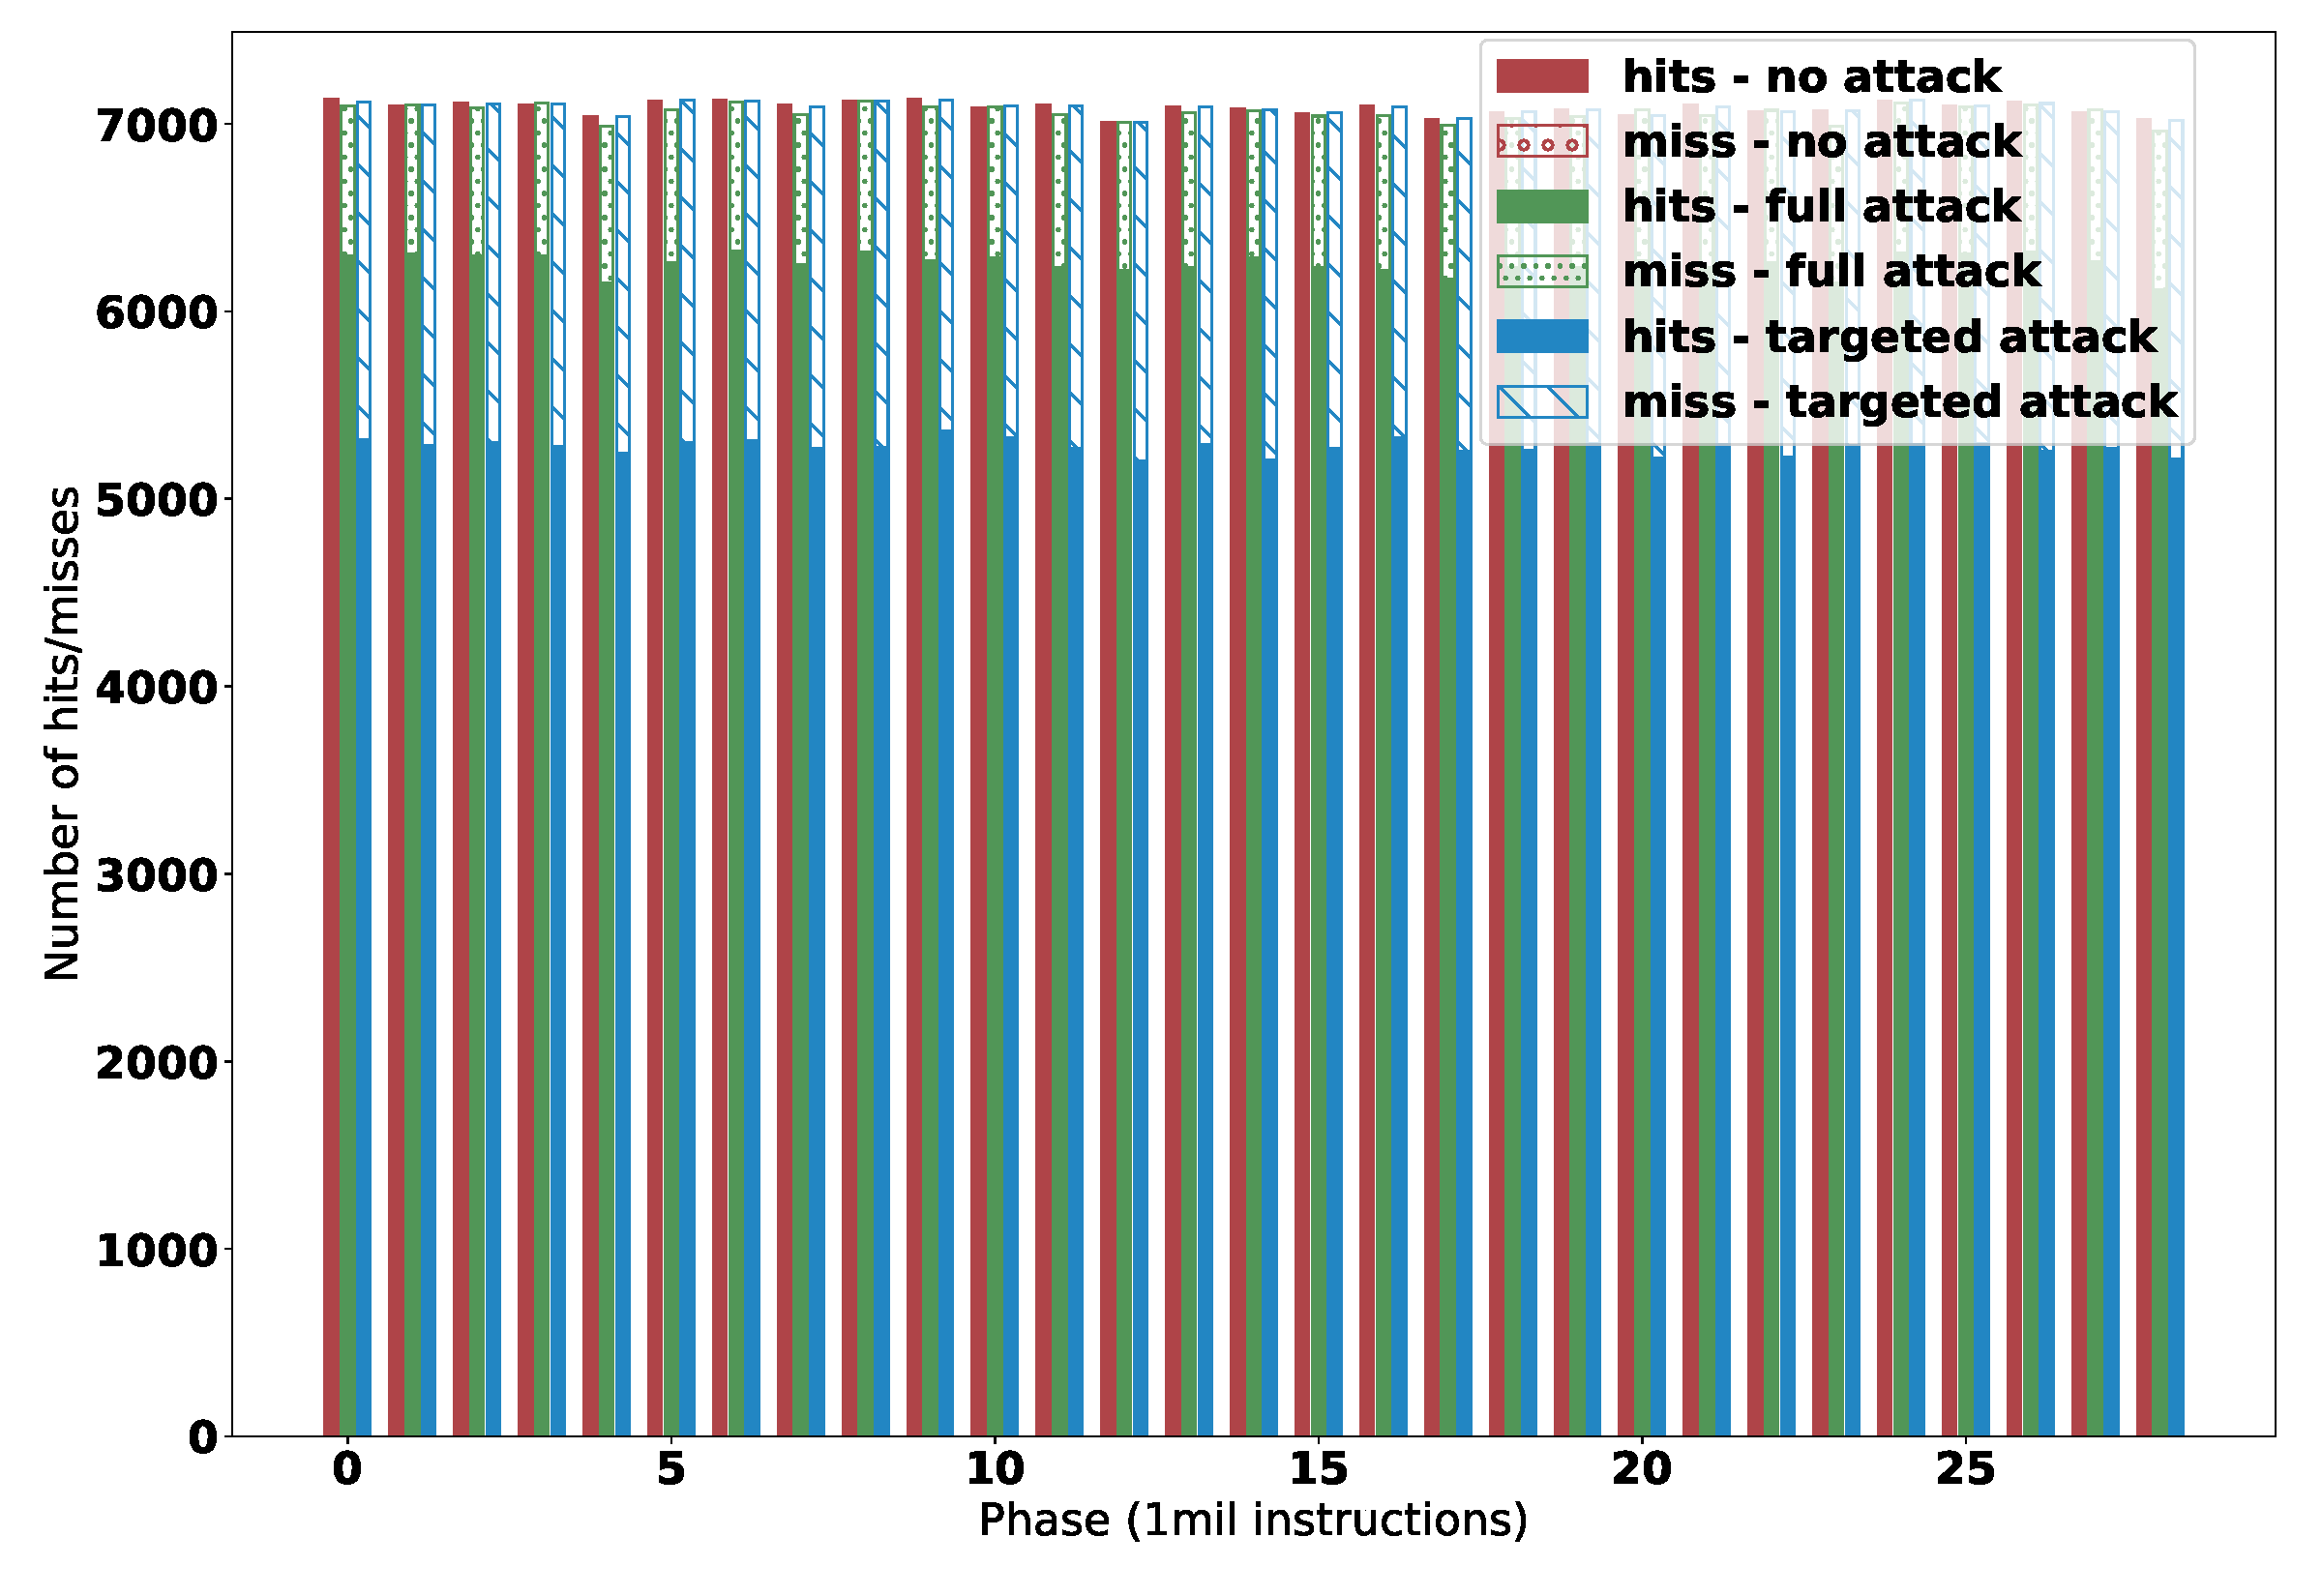
\includegraphics[width=\columnwidth]{pf_hits}
    \caption{Comparision of prefetch table hit and miss count by AES program}
    \label{fig:targeted_hitrate}
\end{figure}

 % Number of hits are significantly lower for targeted
The effectiveness of targeted attacker can also be seen in Figure \ref{fig:targeted_hitrate}
as it is able to double the miss rate of the victim program.

\textbf{DCPT prefetcher:}
 % Same implementation works very well for DCPT.
The same full attacker implementation is tested with a DCPT prefetcher.
A DCPT Prefetcher\cite{dcpt} is a PC indexed table which uses history buffers to
stores deltas of every memory address instead of a single stride value.
The history is then used to predict future deltas. A 128 entry fully associative
table is added instead of the stride prefetcher in the same setup described
in Table \ref{tab:simulation_setup}.
 % Full attacker works better, why ?
Figure \ref{fig:dcpt_hwpf} shows that the full attacker is able to reduce
the number of prefetches by 99\%. This is because of the random strides
generated by the attacker which fill up history buffers of each entry with
irrelevant info. The victim's pattern does not get enough time to be recorded
completely.

\begin{figure}[htbp]
    \centering
    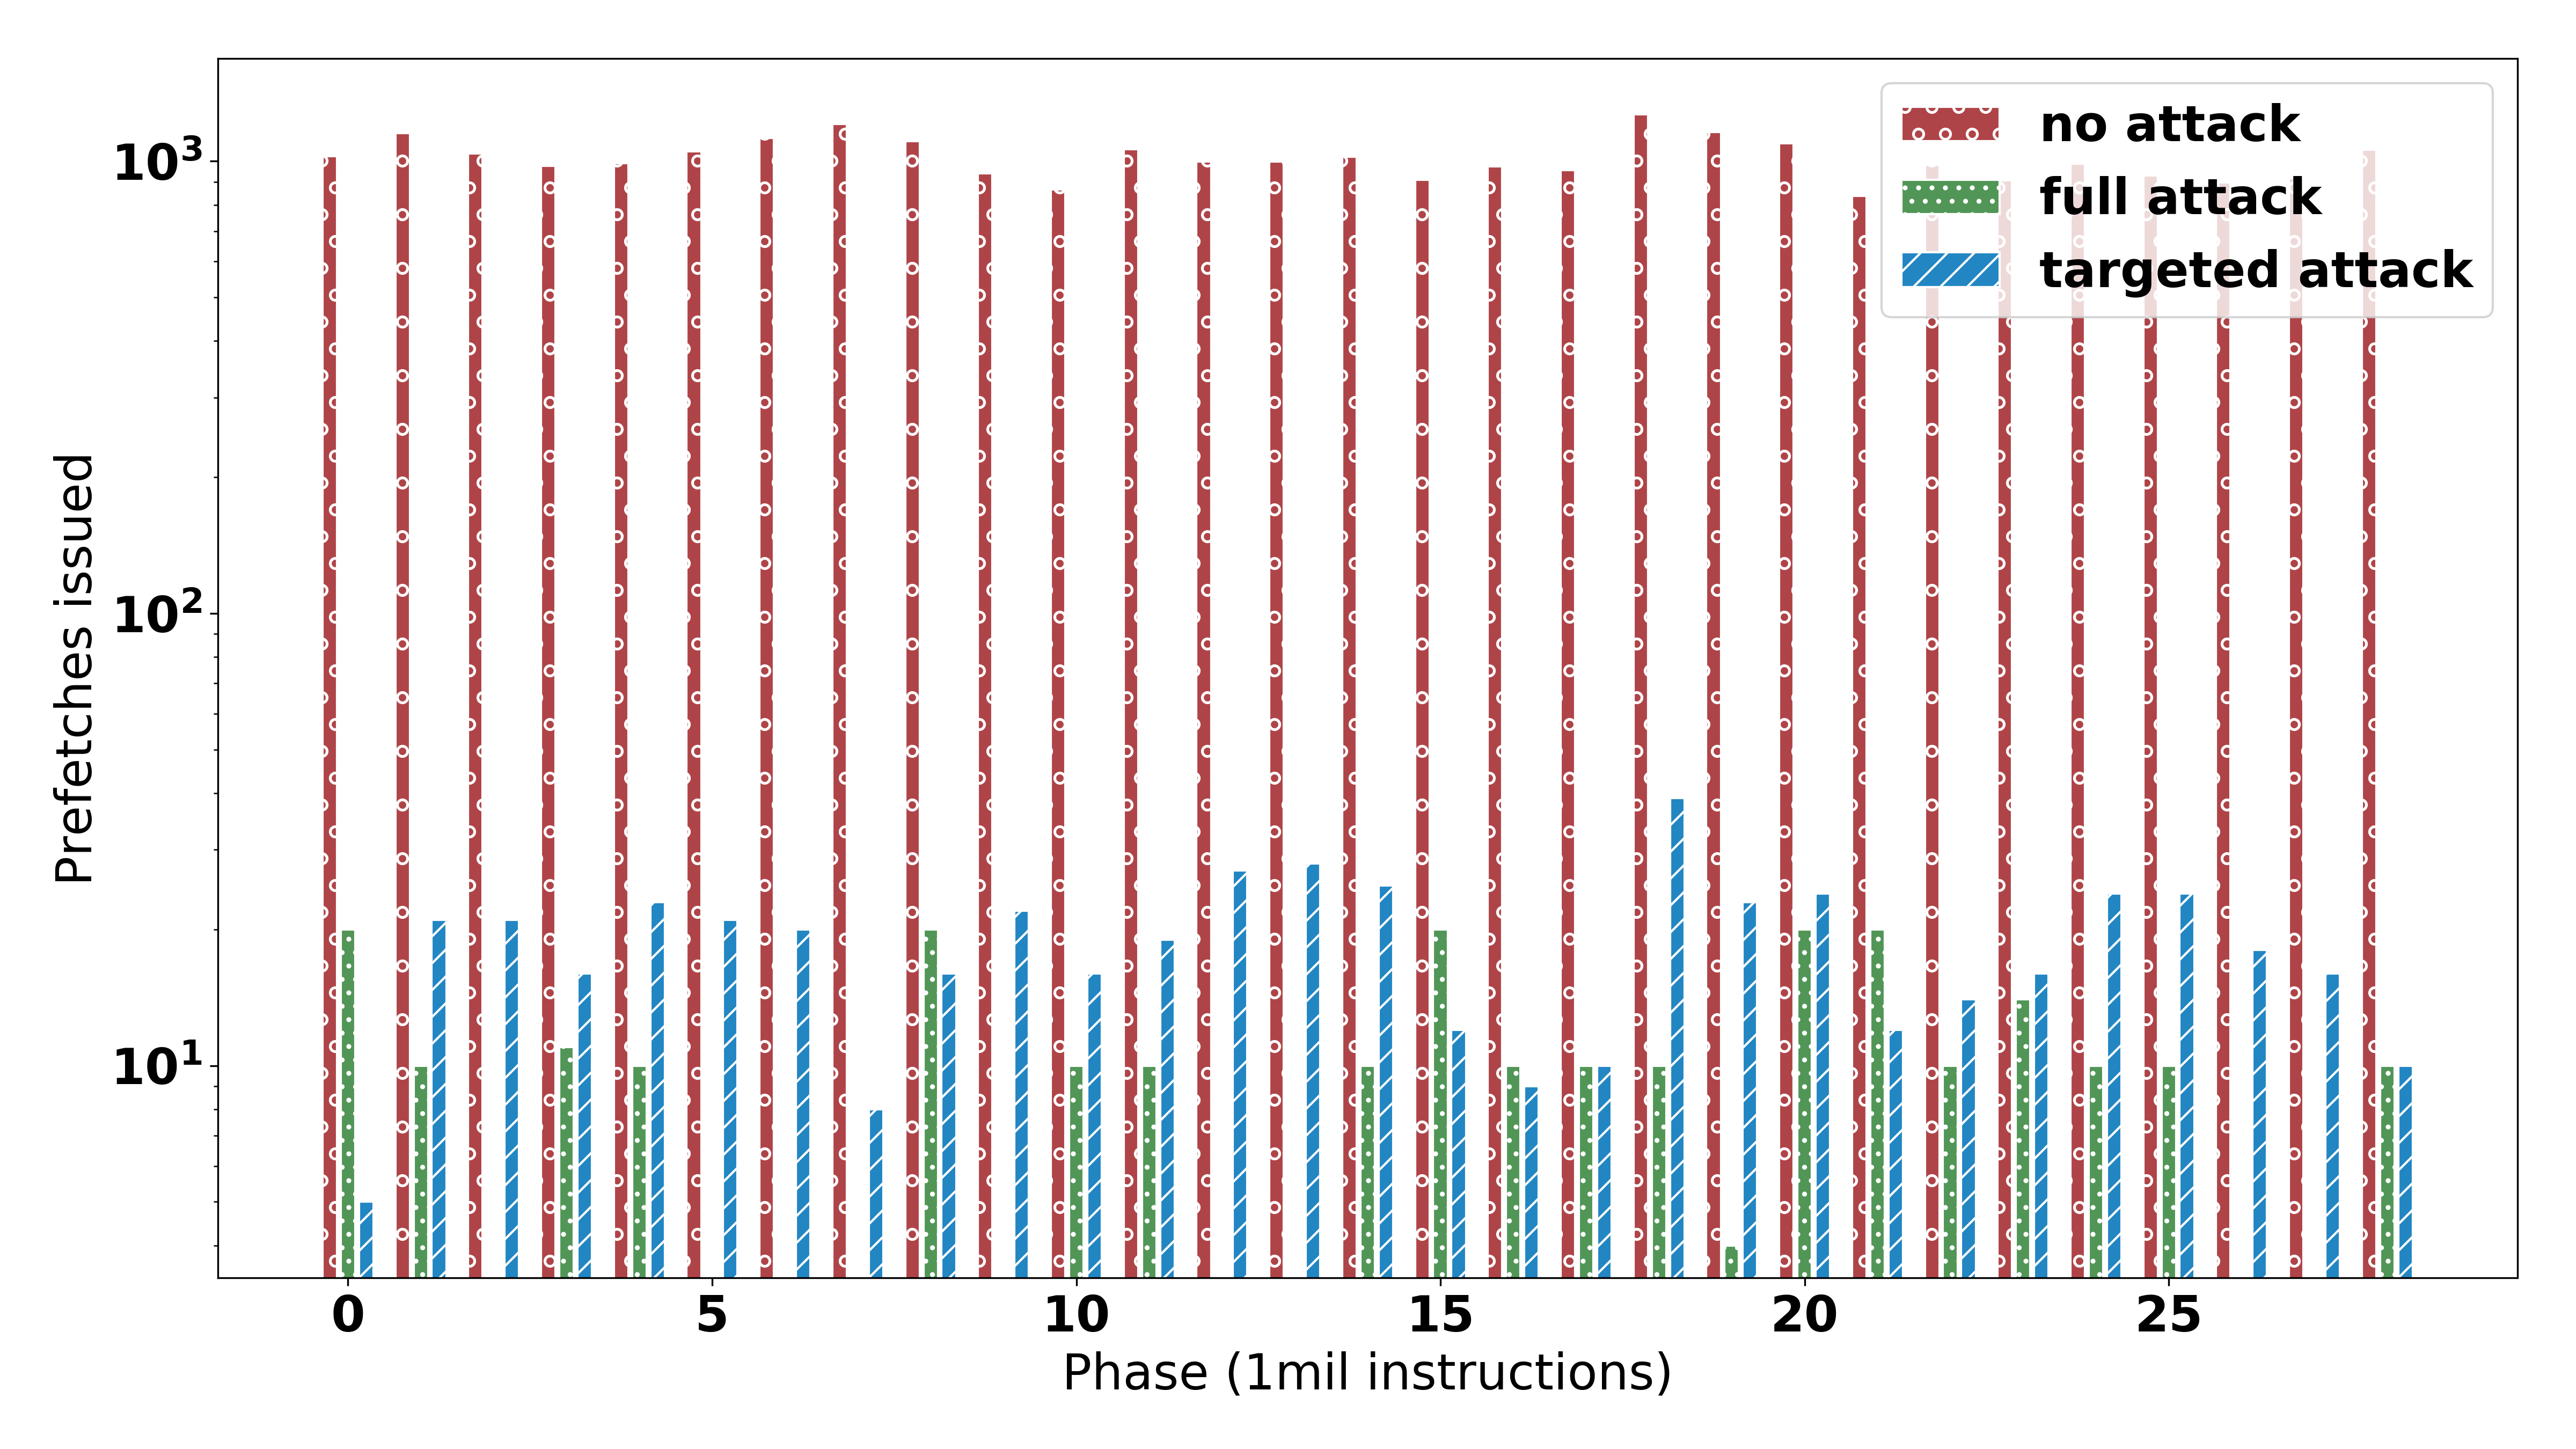
\includegraphics[width=\columnwidth]{dcpt-hwpf}
    \caption{Comparision of number of prefetches issued by DCPT Prefetcher with AES program}
    \label{fig:dcpt_hwpf}
\end{figure}


\section{Conclusion}

The motivation of this work was to disable the prefetcher from
generating memory accesses and prevent it from adding noise
to cache side channels.
The memory access generated by a prefetcher may or may not be eventually
requested by the victim program, hence the prefetcher causes false
positives in a cache side channel.
When the prefetcher is disabled, the system becomes equivalent to
that with no prefetcher present and side channels are amplified.
This paper presents two implementations of an attack on the prefetcher.
An analysis of the working of a stride prefetcher presents
two attack vectors which can be exploited for an attack.
Stride prefetchers use the confidence counter of a valid entry in the
table to generate prefetches. The attacker is designed such that
valid entries of the victim program are regularly evicted from the table,
and the confidence of these entries is not allowed to cross the threshold.

The full attacker is designed to work on the whole prefetcher table.
It is only able to reduce the number of prefetches issued by 32\% for the
AES victim program. The inefficiency of the full attacker is improved
in the targeted attacker which only attacks specific entries of the victim
program. These entries are identified beforehand by running simulations
and the targeted attacker is constructed to target these entries.
The targeted attacker is able to reduce the number of prefetches issued to
0. The reason of this significantly better performance can be seen
in the plots of average confidence and hit rate.

The full attacker is also tried on a DCPT prefetcher having a fully associative
table of 128 entries. The attacker gives a reduction of 99\% in number of prefetches
issued. However, it is not able to reduce the number to completely 0.

\section{Future Scope}

There is scope to build a better attacker which is tailored for history-buffer
based prefetchers like the DCPT prefetcher.
Further tests can be run by testing the attacker in parallel with a side
channel prime+probe attacker to see the impact. The effectiveness of this
attacker on ciphers apart from AES also can be explored.
A similar analysis of security-oriented prefetcher designs, e.g. the Disruptive prefetcher,
can be conducted. It may expose certain weaknesses of the design.



%\section*{Acknowledgment}

%\section*{References}

%\begin{thebibliography}{00}
%\end{thebibliography}
\bibliography{main}
\bibliographystyle{ieeetr}

\end{document}
